\section{The SecureFlow module}\label{sec:flow}
Software usually manipulates information with different security policies. For instance, passwords are sensitive data, while names or birth dates are not. During execution sometimes we want to be sure sensitive information doesn't flow to insecure or public output channels. On the other hand, usually we have to perform some operations with reserved data: this is often done declassifying information. \\
The goal with \texttt{SecureFlow} is to ensure information flow security and declassification policies at compile-time, so that if a code is correctly compiled there are no certain security violations. \\
\citeauthor{russo2008library} \cite{russo2008library} have developed a monadic approach, but their intensive use of the \texttt{IO} monad makes their solution not fully static. In this section I lightly build their work up removing any \texttt{IO} reference. For the sake of simplicity I don't give a discussion about how this can enforce security properties on files or any other data storage mechanism.

\subsection{Security lattice}
\texttt{SecureFlow} is based on a lattice structure, first introduced by \citeauthor{denning1976lattice} \cite{denning1976lattice}, and represented in this library as a type family \cite{kiselyov2010fun}. Security levels are associated to data in order to establish their degree of confidentiality. The lattice ordering relation, written $\sqsubseteq$, represents allowed flows. For instance, $l_{1} \sqsubseteq l_{2}$ indicates that information at security level $l_{1}$ may flow into entities of security level $l_{2}$. In this paper the lattice is implemented like a ticketing system. Listing~\ref{lst:lattice} shows the \texttt{Lattice} module. 
\begin{lstlisting}[caption={The Lattice module}, label={lst:lattice}, breaklines=true]
type family LEQ sl sh :: Constraint
data Ticket s = Ticket
\end{lstlisting}
Basically, \texttt{LEQ}, as a type family, represents a partial function at the type level. Applying the function to parameters (called \textit{type indices}) yields a type. Type families permit a program to compute what data constructors it will operate on, rather than having them fixed statically. Here, LEQ means \textit{Less or Equal}. Trusted programmers are asked to instantiate it specifying the real security lattice. A three level lattice example is shown in Listing~\ref{lst:3lvs}.
\begin{lstlisting}[caption={Three levels lattice}, label={lst:3lvs}, breaklines=true]
module ThreeLevels (Low, Medium, High, low, medium) where

data Low    = L
data Medium = M
data High   = H

type instance (LEQ Low Low)       = ()
type instance (LEQ Low Medium)    = ()
type instance (LEQ Low High)      = ()
type instance (LEQ Medium Medium) = ()
type instance (LEQ Medium High)   = ()
type instance (LEQ High High)     = ()

low :: Ticket Low
low = Ticket

medium :: Ticket Medium
medium = Ticket

high :: Ticket High
high = Ticket
\end{lstlisting}
Here, \texttt{Low}, \texttt{Medium} and \texttt{High} are singleton types (\cite{stone2000singleton}, \cite{pierce2005advanced}). Basically, singleton types are those which have only one value. Thus, the value of a singleton type has a unique type representing the value. A type theory that allows types to be parameterised by values (like the one adopted by Haskell) can use singleton types to let types depend on singleton values. The sequence of \texttt{type instance} allows programmers to specify the relations among \texttt{Low}, \texttt{Medium} and \texttt{High}. Listing~\ref{lst:3lvs} shows also a ticketing system instance. Tickets are generally used as a level proof. Note that the \texttt{high} ticket is not exported, so that one may get access to high secure data only according to the declassification policies. The ordering relation among \texttt{Low}, \texttt{Medium} and \texttt{High} is the following: $Low \sqsubseteq Medium \sqsubseteq High$.

\subsection{SecureFlow Implementation}
Basically, \texttt{SecureFlow} is just an identity monad instance tagged with a proposition allowing access to its value. Actually, that proposition is just a ticket. Listing~\ref{lst:secureflow} shows the module.
\begin{lstlisting}[caption={SecureFlow monad}, label={lst:secureflow}, breaklines=true]
data SecureFlow s a = SF a
type Hatch s a b = SecureFlow s (a -> b)

instance Functor (SecureFlow s) where
  fmap f (SF x)  = SF $ f x

instance Applicative (SF s) where
  pure x            = SF x
  (SF f) <*> (SF x) = SF $ f x

instance Monad (SecureFlow s) where
  return            = pure
  (Allowed a) >>= f = f a
  
open :: LEQ s s' => Ticket s' -> SecureFlow s a -> a

up :: LEQ s s' => SecureFlow s a -> SecureFlow s' a

declassifyWith :: (LEQ s k, LEQ s' s) => Hatch k a b -> SecureFlow s a -> SecureFlow s' b
\end{lstlisting}
%\begin{frame}{Functor}
	\begin{itemize}
		\item Values can be encapsulated in contexts
		\item Applying a function yields different results depending on the context
	\end{itemize}
	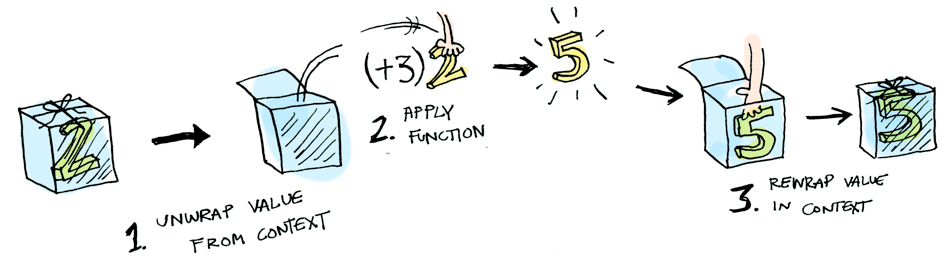
\includegraphics[scale=0.33]{fmap}
	\begin{itemize}
		\item<2-> Generic functions on contexts!
	\end{itemize}
\end{frame}
%\begin{proposition}
\texttt{SecureFlow}, as defined, is an applicative functor.
\end{proposition}
\begin{proof}
We are to prove the four applicative laws.
\begin{enumerate}
	\item \textbf{Identity}: \texttt{pure id <*> v = v}
	\item \textbf{Homomorphism}: \\ \texttt{pure f <*> pure x = pure (f x)}
	\item \textbf{Interchange}: \\ \texttt{u <*> pure y = pure (\$ y) <*> u}
	\item \textbf{Composition}: \texttt{pure (.) <*> u <*> v <*> w = u <*> (v <*> w)}
\end{enumerate}
\end{proof}
\begin{proposition}
\texttt{SecureFlow}, as defined, is a monad.
\end{proposition}
\begin{proof}
I am to prove the three monad laws. 
\begin{enumerate}
	\item \textbf{Left identity}: \texttt{return a >>= f = f a}
		\begin{lstlisting}
(return a >>= f) = (pure a >>= f) = 
= ((SF a) >>= f) = f a
		\end{lstlisting}
	
	\item \textbf{Right identity}: \texttt{m >>= return = m}
		\begin{lstlisting}
((SF a) >>= return) = 
= (return a) = (pure a) = 
= (SF a) = m
		\end{lstlisting}
	\item \textbf{Associativity}: \texttt{(m >>= f) >>= g = m >>= ($\backslash$x -> f x >>= g)} 
		\begin{lstlisting}
(((SF a) >>= f) >>= g) = 
= ((f a) >>= g) = (g (f a))

(SF a >>= (\x -> f x >>= g)) =
= (\x -> f x >>= g) a = 
= ((f a) >>= g) = (g (f a))
		\end{lstlisting}
\end{enumerate}
\texttt{SecureFlow} satisfies the three monad laws, hence it is a monad.
\end{proof}
\texttt{SecureFlow} is also a functor and an applicative. The proof is largely similar to the last one, so it is omitted. \\
The module also exports three important functions, \texttt{up}, \texttt{open} and \texttt{declassifyWith}. \\
\texttt{open} is used to look at a protected value of type \texttt{SecureFlow s a}. However, in order to do that, one has to prove to have a value of type \texttt{s}. This proof is given with the ticketing system. Note that, if the value is protected with \texttt{SecureFlow s a}, the ticket type must be in the \texttt{LEQ} relation with \texttt{s}. This actually means $s \sqsubseteq s'$ must hold. Otherwise the compiler gives a type error because of the unsatisfied type constraint \texttt{LEQ s s'}. \\
The function \texttt{up} can be used to turn any protected value into a protected value at a higher security level. Basically it acts like a cast function from a lower to a higher level. 
\subsection{Declassification}
Non-interference is a security policy which specifies the absence of information flows from secret to public data. So far, the provided library has followed strictly this policy. However, real-word applications release some information as part of their intended behavior. Non-interference does not provide any way to distinguish between such releases of information and those ones produced by malicious code, programming errors or vulnerability attacks. Consequently, relaxing the notion of non-interference is necessary, considering declassification policies as intended ways to leak information. \\
\citeauthor{sabelfeld2005dimensions} \cite{sabelfeld2005dimensions} have provided a classification of those policies. Basically, each dimension represents a specific policy aspect corresponding to \textit{what}, \textit{where}, \textit{when} and by \textit{whom} data is released. Researchers have defined type systems for enforcing these aspects (\cite{banerjee2008expressive}, \cite{zdancewic2001robust}, \cite{zdancewic2003type}), but their encoding into this work would considerably increase its complexity. This is why here I provide a \textit{declassification combinator}, \texttt{Hatch}, which allows trusted programmers to compose and create declassification policies from scratch. Those policies are based on the \texttt{SecureFlow} monad, hence a statical type check is done on them. In this way, declassification still lies on the non-interference idea, but untrusted programmers are allowed to work with secret data without producing leaks. Furthermore, only trusted programmers are authorised to write them. \\
Basically, \texttt{Hatch} is just a \textit{SecureFlow}-encapsulated function of type \texttt{a -> b}. \texttt{declassifyWith} simply applies that function to the actual value and returns a new value with a lower security level. In order to work, the relation $s' \sqsubseteq s \sqsubseteq k$ must hold. It is such that the final security tag will be \textit{LEQ} than the original one. \\
Listing~\ref{lst:login} shows a login function.
\begin{lstlisting}[caption={Declassificated login}, label={lst:login}]
login :: String -> String -> 
  Hatch High [Credential] Bool
login e p = pure
  (\cs -> elem (Credential e p) cs)


check = (declassifyWith (login e p) cs)
  :: SecureFlow Medium Bool
success = open medium check
\end{lstlisting}
Basically \texttt{Credential} represents the pair \textit{(email address, password)}, and it is tagged with the \textit{High} level. \texttt{login} simply takes a list of \textit{Credentials} and checks for a match with the provided email address and password. Note that \texttt{High} in \texttt{login} type signature refers to the list security level rather than to the final one. The latter is code provided giving an explicit type to the \texttt{declassifyWith} result (in this case, \textit{Medium}, forced by \texttt{:: SecureFlow Medium Bool}). With a \texttt{medium} ticket we shall be able to access the boolean value and check whether or not the user is actually allowed to login. That would not be possible without declassifying \textit{Credentials} list. \\
Listing~\ref{lst:salary} shows how a sensitive salary could be declassified, for instance, for test purposes.
\begin{lstlisting}[caption={Declassificated salary}, label={lst:salary}]
-- Employee model would be like the 
-- following:
-- { firstName  :: SecureFlow Low String
-- , lastName   :: SecureFlow Low String
-- , birthdate  :: SecureFlow Low String
-- , salary     :: SecureFlow High Int
-- , email      :: SecureFlow Medium String
-- , leader     :: SecureFlow Low Bool
-- }

showSalary :: Hatch High Int Int
showSalary = pure id 
\end{lstlisting}
This model specifies a \textit{High} level for \texttt{salary}, but thanks to \texttt{showSalary} a declassification to another security level \textit{l}, where $l \sqsubseteq High$, would be possible. \\
Two other important things are, finally, pointed out by this example. First, \texttt{SecureFlow} may be applied both for an entire module (like \textit{Credential} before), or with a more fine granularity, as in \textit{Employee}. Second, declassification functions are extremely sensitive and only trusted programmers ought to write them. However, remembering my assumptions, only trusted programmers are supposed to ''instantiate'' the secure library, so that once they have defined declassification policies no one will be able to modify them. Otherwise there would be no way to ensure information flow security with this kind of approach.